\section{Introduction}

\subsection{Reasons of trade}
\begin{itemize}
    \item \textbf{Countries' differences: comparative advantage}
    \begin{itemize}
        \item Productivity: Ricardo
        \item Endowments: Heckscher-Ohlin
    \end{itemize}
    \item \textbf{Countries' similarities: economies of scale}
\end{itemize}

\subsection{Comparative advantage}
\begin{note}
    \

    Stanislaw Ulam's challenge to Paul Samuelson:  ``name me one
proposition in all of the social sciences which is both true and
non-trivial''. 

Samuelson's answer: Comparative advantage. ``That it is logically true need not be
argued before a mathematician; that is is not trivial is attested by
the thousands of important and intelligent men who have never
been able to grasp the doctrine for themselves or to believe it after
it was explained to them.''.\footnote{P.A. Samuelson (1969), ``The Way of an Economist,'' 
in P.A. Samuelson, ed., International Economic Relations: Proceedings of the Third Congress of the
International Economic Association, Macmillan: London, pp. 1-11.}
\end{note}

In the simplest and earliest complete model of production and trade,
the reason for trade is \textbf{comparative advantage}.
And the source of comparative advantage is \textbf{differences in production technologies}.

These are the differnces in production functions, not the differences
in labor productivities due to different endowments of capital which is the type of 
Heckscher-Ohlin model.

\subsection{Basic assumptions}
\begin{itemize}
    \item Labor is the only factor of production
    \item Constant returns to scale
    \item Perfect competition
    \item Full employment
    \item Endowments given, confined to country but intersectorally mobile
    within each country
    \item Two countries with different technologies (production functions)
    \item Number of goods: $n \geq 2$
\end{itemize}

\subsection{Technology}

\begin{question}
    How is efficiency measured?
\end{question}
With only one factor, we measure by the usage of the factor: \textbf{labbor requirement per unit output}.

We define the quantity of labour (e.g. number of hours) necessary
to produce one unit of good $i$ as $a_i$. If $a_i=2$, it means that 2 hours of labor
are needed to produce one unit of good $i$.

So, the labor productivity is the inverse of the labor requirement $a_i$, the higher the labor requirement, the lower the productivity.

\subsection{Production Possibility Frontier: Refresher}

PPF is the maximum possible production level for a given technology and factor endowment.
\begin{itemize}
    \item Constraint: points outside the PPF are not feasible;
    \item Efficiency: points inside the PPF are inefficient, those on the PPF are efficient;
    \item Opportunity cost: the slope of the PPF is the opportunity cost of producing one more unit of good $i$ in terms of good $j$.
    \item Concavity: the PPF is usually concave to the origin due to the law of diminishing returns.
\end{itemize}
Technology progress shifts the PPF outwards.

\section{The two-sector Model}

\subsection{A Simple Numerical Example}

Let's begin with a simple example: US and India producing corn and auto.
\begin{table}[htbp!]
    \centering
    \begin{tabular}{c|cc}
        \hline
        & US & India \\
        \hline
        Labor force & $L=200$ & $L^*=800$ \\
        Labor per unit corn & $a_c=8$ & $a_C^*=50$ \\
        Labor per unit auto & $a_A=10$ & $a_A^*=40$ \\
        \hline
    \end{tabular}
\end{table}

Specific assumption of this example : US is more
efficient/productive at producing both goods, meaning
US has an absolute advantage in both goods.

\subsubsection{Production Possibility Frontier}

\begin{minipage}{0.45\textwidth}
    \textbf{US}
    
    The full-employment condition is:
    \[
    L = a_{c}Q_{c} + a_{A}Q_{A}
    \]
    The PPF is a straight line connecting these two points:
    \[
    Q_A = \frac{L}{a_A} - \frac{a_C}{a_A}Q_C
    \]
    \centering
    \begin{tikzpicture}[scale=0.14]
        \draw[->] (0,0) -- (30,0) node[right] {$Q_C$};
        \draw[->] (0,0) -- (0,25) node[above] {$Q_A$};
            
            % PPF line
        \draw[thick, blue] (0,20) -- (25,0) node[midway, above, sloped]{};
            
        \node[below] at (25,0) {$25$};
        \node[left] at (0,20) {$20$};
            
    \end{tikzpicture}
    \captionof{figure}{US PPF}
\end{minipage}
\hfill
\begin{minipage}{0.45\textwidth}
    \textbf{India}
    
    The full-employment condition is:
    \[
    L^* = a_{C}^*Q_{C} + a_{A}^*Q_{A}
    \]

    The PPF is a straight line connecting these two points:
    \[
    Q_A^* = \frac{L^*}{a_A^*} - \frac{a_C^*}{a_A^*}Q_C
    \]
    \centering
    \begin{tikzpicture}[scale=0.14]
        \draw[->] (0,0) -- (30,0) node[right] {$Q_C^*$};
        \draw[->] (0,0) -- (0,25) node[above] {$Q_A^*$};
            
            % PPF line
        \draw[thick, red] (0,20) -- (16,0) node[midway, above, sloped]{};
        
        \node[below] at (16,0) {$16$};
        \node[left] at (0,20) {$20$};
    \end{tikzpicture}
    \captionof{figure}{India PPF}
\end{minipage}

\subsubsection{Relative price and Technology}

\begin{notation}
    \

    Relative price of corn: $P = \frac{P_C}{P_A}$;

    Relative quantity of corn: $Q = \frac{Q_C}{Q_A}$;

    $L$ and $L^*$ are the endowments of labor(in efficient units) in the two countries;

    $w$ and $w^*$ are the wage(in efficiency units) in the two countries.
\end{notation}

Workers are paid the value of their marginal products: $w_C = \frac{P_C}{a_C}$ and $w_A = \frac{P_A}{a_A}$.

Perfectly mobile labor: If both goods are produced, the wage in both sectors must be the same.
\[w_C = w_A \Leftrightarrow P = \frac{a_C}{a_A}.\]

\subsubsection{Production and Supply in the US}

If $P = \frac{a_C}{a_A} = 0.8$, the international price(relative price) is equal to the domestic opportunity cost of producing corn in terms of auto.
Trade cannot bring extra gains. Hence the production set doesn't affect the consumption set, and the production set can be anywhere on the PPF. $1 \leq \frac{Q_c}{Q_A} < \infty$. 

If $P < \frac{a_C}{a_A} = 0.8$, international price of C is lower than the domestic opportunity cost of producing C in terms of A. 
US will produce only A and import C. 
$Q_C = 0$, $Q_A = 20$, and $\frac{Q_C}{Q_A} = 0$.

If $P > \frac{a_C}{a_A} = 0.8$, international price of C is higher than the domestic opportunity cost of producing C in terms of A. 
US will produce only C and export A.
$Q_A = 0$, $Q_C = 25$, and $\frac{Q_C}{Q_A} = \infty$.

\begin{center}
\begin{tikzpicture}[scale=1.2]
    % Axes
    \draw[->] (0,0) -- (6,0) node[right] {$\frac{Q_C}{Q_A}$};
    \draw[->] (0,0) -- (0,4) node[above] {$P = \frac{P_C}{P_A}$};
    
    % Critical price line
    \draw[dashed] (0,1.6) -- (5.5,1.6) node[left] at (0,1.6) {$0.8 = \frac{a_C}{a_A}$};
    
    % Supply curve
    \draw[thick, blue] (0,0) -- (0,1.6) -- (5,1.6) -- (5,4);
    
    % Points for clarification
    \fill[blue] (0,1.6) circle (2pt);
    \fill[blue] (5,1.6) circle (2pt);
    
    % Labels
    \node[blue, left] at (0,0.8) {Only Autos ($Q_C=0, Q_A=20$)};
    \node[blue, below] at (2.5,1.6) {Both goods produced};
    \node[blue, right] at (5,2.5) {Only Corn ($Q_C=25, Q_A=0$)};
    
    % X-axis markers
    \node[below] at (0,0) {$0$};
    \node[below] at (5,0) {$\infty$};
\end{tikzpicture}
\captionof{figure}{US Relative supply}
\end{center}

\subsubsection{Autarky equilibria in the two countries}

\begin{minipage}{0.48\textwidth}
    \centering
    \begin{tikzpicture}[scale=1.2]
        % Axes
        \draw[->] (0,0) -- (4,0) node[right] {$\frac{Q_C}{Q_A}$};
        \draw[->] (0,0) -- (0,3) node[above] {$P = \frac{P_C}{P_A}$};
        
        % Critical price line
        \draw[dashed] (0,0.8) -- (3.7,0.8) node[left] at (0,0.8) {$0.8 = \frac{a_C}{a_A}$};
        
        % Supply curve
        \draw[thick, blue] (0,0) -- (0,0.8) -- (3.2,0.8) -- (3.2,2.8);
        
        % Points for clarification
        \fill[blue] (0,0.8) circle (2pt);
        \fill[blue] (3.2,0.8) circle (2pt);
        
        % Labels
        \node[blue, left, scale=0.7] at (0,0.4) {Only Autos};
        \node[blue, above, scale=0.7] at (1.6,0.8) {Both goods};
        \node[blue, right, scale=0.7] at (3.2,2) {Only Corn};
        
        % X-axis markers
        \node[below] at (0,0) {$0$};
        \node[below] at (5,0) {$\infty$};
    \end{tikzpicture}
    \captionof{figure}{US Relative Supply}
\end{minipage}
\hfill
\begin{minipage}{0.48\textwidth}
    \centering
    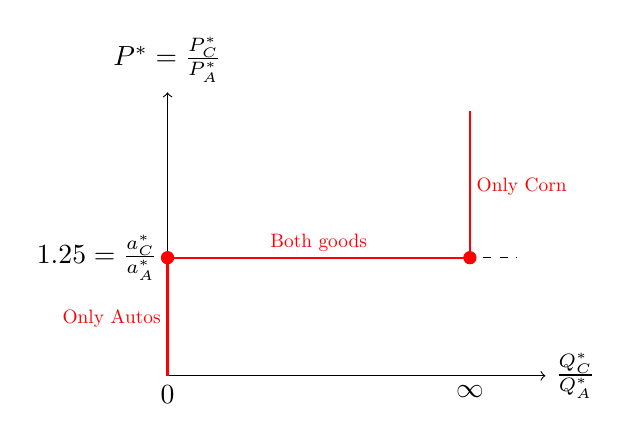
\begin{tikzpicture}[scale=1.2]
        % Axes
        \draw[->] (0,0) -- (4,0) node[right] {$\frac{Q_C^*}{Q_A^*}$};
        \draw[->] (0,0) -- (0,3) node[above] {$P^* = \frac{P_C^*}{P_A^*}$};
        
        % Critical price line
        \draw[dashed] (0,1.25) -- (3.7,1.25) node[left] at (0,1.25) {$1.25 = \frac{a_C^*}{a_A^*}$};
        
        % Supply curve
        \draw[thick, red] (0,0) -- (0,1.25) -- (3.2,1.25) -- (3.2,2.8);
        
        % Points for clarification
        \fill[red] (0,1.25) circle (2pt);
        \fill[red] (3.2,1.25) circle (2pt);
        
        % Labels
        \node[red, left, scale=0.7] at (0,0.6) {Only Autos};
        \node[red, above, scale=0.7] at (1.6,1.25) {Both goods};
        \node[red, right, scale=0.7] at (3.2,2) {Only Corn};
        
        % X-axis markers
        \node[below] at (0,0) {$0$};
        \node[below] at (3.2,0) {$\infty$};
    \end{tikzpicture}
    \captionof{figure}{India Relative Supply}
\end{minipage}

\subsubsection{Trade: Relative supply}

When we combine the two countries to form the world market, we get the following relative supply curve:

- When $P<0.8$, both countries produce only autos, world ratio $R = 0$.

- When $P=0.8$, US can vary production between 20 autos, 
no corn (world $R = 0$), and 0 autos, 25 corn (world
$R = 1.25$) while India produces only autos, so world $R \in [0, 1.25]$.

- When $0.8<P<1.25$, US produces only corn, India produces only autos, so $R = \frac{25}{20} = 1.25$.

- When $P=1.25$, India can vary production while US produces only corn, so world $R \in \left. \left[ 1.25, \infty \right. \right)$.

- When $P>1.25$, both countries produce only corn, so world $R = \infty$.

\begin{center}
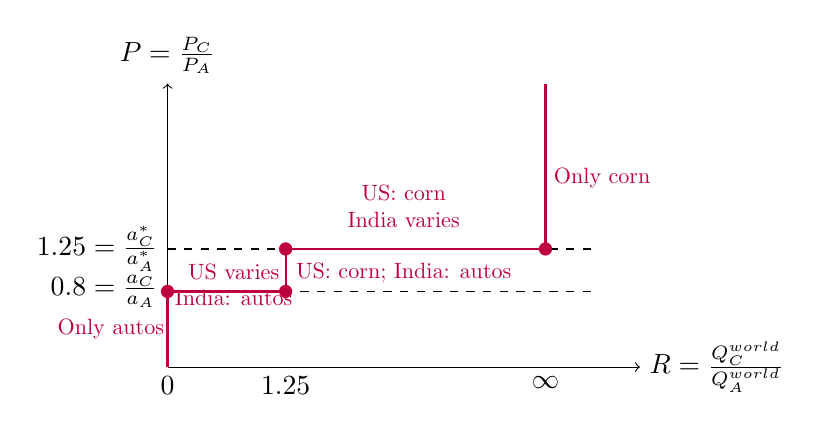
\begin{tikzpicture}[scale=1.2]
    % Axes
    \draw[->] (0,0) -- (5,0) node[right] {$R = \frac{Q_C^{world}}{Q_A^{world}}$};
    \draw[->] (0,0) -- (0,3) node[above] {$P = \frac{P_C}{P_A}$};
    
    % Critical price lines
    \draw[dashed] (0,0.8) -- (4.5,0.8) node[left] at (0,0.8) {$0.8 = \frac{a_C}{a_A}$};
    \draw[dashed] (0,1.25) -- (4.5,1.25) node[left] at (0,1.25) {$1.25 = \frac{a_C^*}{a_A^*}$};
    
    % World Relative Supply curve
    \draw[thick, purple] (0,0) -- (0,0.8) -- (1.25,0.8) -- (1.25,1.25) -- (4,1.25) -- (4,3);
    
    % Points for clarification
    \fill[purple] (0,0.8) circle (2pt);
    \fill[purple] (1.25,0.8) circle (2pt);
    \fill[purple] (1.25,1.25) circle (2pt);
    \fill[purple] (4,1.25) circle (2pt);
    
    % Region labels
    \node[purple, scale=0.8, align=left] at (-0.6,0.4) {Only autos};
    \node[purple, scale=0.8, align=center] at (0.7,0.87) {US varies\\India: autos};
    \node[purple, scale=0.8, align=center] at (2.5,1) {US: corn; India: autos};
    \node[purple, scale=0.8, align=center] at (2.5,1.7) {US: corn\\India varies};
    \node[purple, scale=0.8, align=right] at (4.6,2) {Only corn};
    
    % X-axis markers
    \node[below] at (0,0) {$0$};
    \node[below] at (1.25,0) {$1.25$};
    \node[below] at (4,0) {$\infty$};
\end{tikzpicture}
\captionof{figure}{World Relative Supply Curve}
\end{center}

\subsubsection{Trading Equilibrium}

Depending on position of relative demand, the trading equilibrium can be one of three types:
\begin{itemize}
    \item[A.] $P=0.8$, US produces both goods, India produces only autos;
    \item[B.] $0.8<P<1.25$, US produces only corn, India produces only autos;
    \item[C.] $P=1.25$, US produces only corn, India produces both goods.
\end{itemize}

\begin{center}
    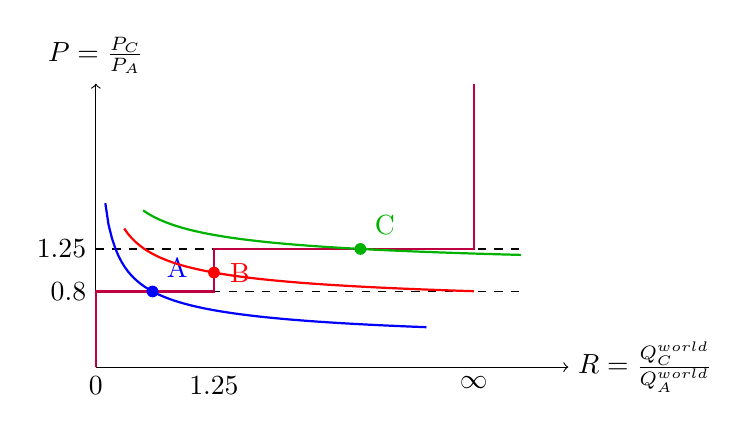
\begin{tikzpicture}[scale=1.2]
        % Axes
        \draw[->] (0,0) -- (5,0) node[right] {$R = \frac{Q_C^{world}}{Q_A^{world}}$};
        \draw[->] (0,0) -- (0,3) node[above] {$P = \frac{P_C}{P_A}$};
        
        % Critical price lines
        \draw[dashed] (0,0.8) -- (4.5,0.8) node[left] at (0,0.8) {$0.8$};
        \draw[dashed] (0,1.25) -- (4.5,1.25) node[left] at (0,1.25) {$1.25$};
        
        % World Relative Supply curve
        \draw[thick, purple] (0,0) -- (0,0.8) -- (1.25,0.8) -- (1.25,1.25) -- (4,1.25) -- (4,3);
        
        % New equilibrium points (adjusted)
        \node[circle, fill, blue, inner sep=1.5pt, label={[blue]above right:A}] at (0.6,0.8) {};
        \node[circle, fill, red, inner sep=1.5pt, label={[red]right:B}] at (1.25,1.0) {};
        \node[circle, fill, green!70!black, inner sep=1.5pt, label={[green!70!black]above right:C}] at (2.8,1.25) {};
        
        % Indifference curves (parallel)
        % Curve A passing through (0.6,0.8)
        \draw[blue, thick] plot[domain=0.1:3.5, samples=100] (\x, {0.5 * pow(\x, -0.5) + 0.1545});
        
        % Curve B passing through (1.25,1.0)
        \draw[red, thick] plot[domain=0.3:4, samples=100] (\x, {0.5 * pow(\x, -0.5) + 0.5528});
        
        % Curve C passing through (2.8,1.25)
        \draw[green!70!black, thick] plot[domain=0.5:4.5, samples=100] (\x, {0.5 * pow(\x, -0.5) + 0.9512});
        
        % X-axis markers
        \node[below] at (0,0) {$0$};
        \node[below] at (1.25,0) {$1.25$};
        \node[below] at (4,0) {$\infty$};
    \end{tikzpicture}
    \captionof{figure}{Trading Equilibrium}
\end{center}

\subsubsection{Efficient production and world PPF}

Suppose initially all labor produc autos in both: 40 in all.
If any corn is produced, it's better to do so by switching sone labor in the US:
because wach auto not produced releases 10 labor which can then produce 1.25 corn,
while in India, each less auto yields only 0.8 more corn.

Only when all US labor has been diverted to producing corn
should any Indian labor be switched.

Conversely, starting with all corn: 41 units, to produce any autos,
Indian labor should be switched.

This despite the US producing autos more efficiently than India: only
10 units of labor against 40. The reason: the US produces corn even
more efficiently: only 8 units of labor against 50. What matters is the
ratio (opportunity cost): $\frac{10}{8} > \frac{40}{50}$, or $\frac{10}{40} > \frac{8}{50}$.

\begin{center}
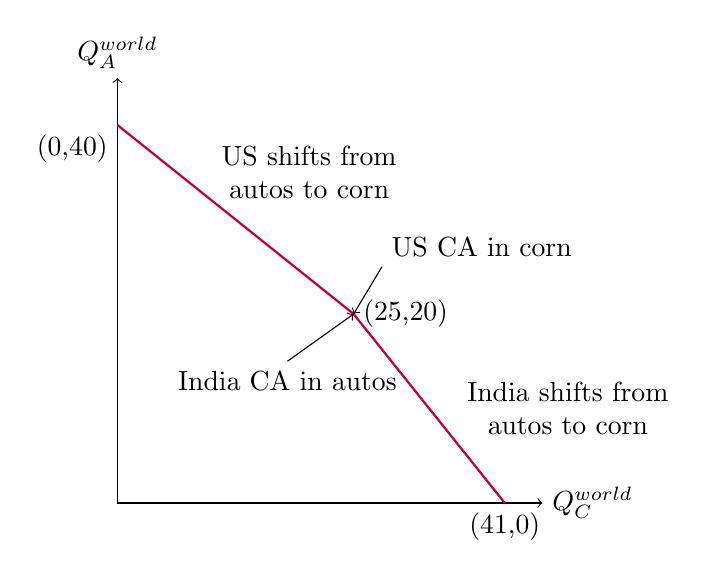
\begin{tikzpicture}[scale=0.12]
    % Axes
    \draw[->] (0,0) -- (45,0) node[right] {$Q_C^{world}$};
    \draw[->] (0,0) -- (0,45) node[above] {$Q_A^{world}$};
    
    % World PPF
    \draw[thick, purple] (0,40) -- (25,20) -- (41,0);
    
    % Points for clarification
    \fill[purple] (0,40) circle (2pt);
    \fill[purple] (25,20) circle (2pt);
    \fill[purple] (41,0) circle (2pt);
    
    % Labels for key points
    \node[below left] at (0,40) {(0,40)};
    \node[right] at (25,20) {(25,20)};
    \node[below] at (41,0) {(41,0)};
    
    % Production allocation labels
    \node[right, align=center] at (10,35) {US shifts from\\autos to corn};
    \node[right, align=center] at (36,10) {India shifts from\\autos to corn};
    
    % Efficiency regions
    \node[below left, purple] at (0,40) {};
    \node[right, purple] at (25,20) {};
    \node[above right, purple] at (41,0) {};
    
    % Country labels for the kink point
    \draw[->] (28,25) -- (25,20);
    \node[above right] at (28,25) {US CA in corn};
    \draw[->] (18,15) -- (25,20);
    \node[below] at (18,15) {India CA in autos};
\end{tikzpicture}
\captionof{figure}{World Production Possibility Frontier}
\end{center}

\subsubsection{TRading equilibrium and world PPF}

If preferences are identical and homthetic everywhere, we can draw the world indifference curves.
Depending on their shape, there are three types of outcomes:
\begin{itemize}
    \item[A.] US produces both goods, India produces only autos;
    \item[B.] US produces only corn, India produces only autos;
    \item[C.] US produces only corn, India produces both goods.
\end{itemize}

Relative price of corn $=$ slope of PPF: 0.8 in A, 1.25 in C, between 0.8 and 1.25 in B.

\begin{center}
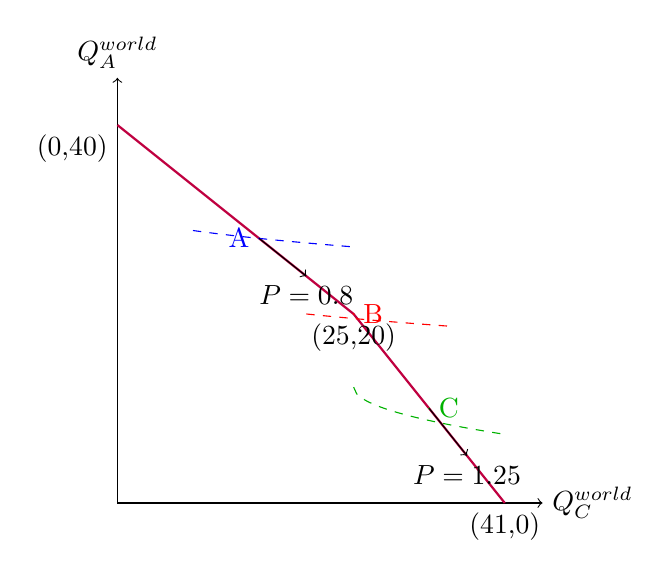
\begin{tikzpicture}[scale=0.12]
    % Axes
    \draw[->] (0,0) -- (45,0) node[right] {$Q_C^{world}$};
    \draw[->] (0,0) -- (0,45) node[above] {$Q_A^{world}$};
    
    % World PPF
    \draw[thick, purple] (0,40) -- (25,20) -- (41,0);
    
    % Equilibrium points
    \fill[blue] (15,28) circle (3pt) node[left] {A};
    \fill[red] (25,20) circle (3pt) node[right] {B};
    \fill[green!70!black] (33,10) circle (3pt) node[right] {C};
    
    % Indifference curves
    \draw[blue, dashed] plot[domain=8:25, samples=50] (\x, {31.1 - 0.8*sqrt(\x)});
    \draw[red, dashed] plot[domain=20:35, samples=50] (\x, {23.1 - 0.8*sqrt(\x-5)});
    \draw[green!70!black, dashed] plot[domain=25:41, samples=50] (\x, {12.263 - 1.25*sqrt(\x-25)});
    
    % Labels for key points
    \node[below left] at (0,40) {(0,40)};
    \node[below] at (25,20) {(25,20)};
    \node[below] at (41,0) {(41,0)};
    
    % Production allocations
    \node[blue, above, align=center] at (15,28) {};
    \node[red, below left, align=center] at (25,20) {};
    \node[green!70!black, above, align=center] at (33,10) {};
    
    % Price lines
    \draw[->, thin] (15,28) -- (20,24);
    \node[below] at (20,24) {$P=0.8$};
    
    % \draw[->, thin] (25,20) -- (30,17);
    % \node[below] at (30,17) {$0.8<P<1.25$};
    
    \draw[->, thin] (33,10) -- (37,5);
    \node[below] at (37,5) {$P=1.25$};
\end{tikzpicture}
\captionof{figure}{Trading Equilibrium on the World PPF}
\end{center}